\documentclass{article}
\usepackage[utf8]{inputenc}
\usepackage[margin=1in]{geometry}
\usepackage{algorithm}
\usepackage{algpseudocode}
\usepackage{graphicx}
\usepackage{fancyhdr}

\AtBeginDocument{%
  \providecommand\BibTeX{{%
    \normalfont B\kern-0.5em{\scshape i\kern-0.25em b}\kern-0.8em\TeX}}}

\newcommand{\code}[1]{\texttt{#1}}

\title{EECS 219B: Formal Methods — Assignment 1}
\author{Parker Ziegler}
\pagestyle{fancy}
\lhead{EECS 219B: Formal Methods — Assignment 1}
\rhead{Parker Ziegler}

\begin{document}

\maketitle

\section{Horn-SAT and Renamable Horn-SAT}

\bigskip
\subsection{A Linear Time Algorithm for Deciding the Satisfiability of HornSAT Formulae}

\bigskip
\noindent We base this algorithm off of the work of Dowling and Gallier \cite{dowling_1984}.

\subsubsection{Data Structures}

\medskip
\noindent Let us assume that we have a HornSAT formula, $\phi$, in CNF. To begin, we initialize a collection of data structures to assist with tracking truth assignments to literals.

\begin{enumerate}
  \item For each positive literal $p$ in $\phi$, we compute a list $cl_p$ containing those clauses in which $p$ appears as a negative literal. Thinking of Horn clasues as implications, this list represents the set of all clauses for which $p$ appears on the left-hand side of an implication.
  \item We compute an array $nls$ such that $nls[c]$ returns the number of negative literals in clause $c$ that have current truth value $false$ (0). A clause $c$ is ready for processing by our algorithm if $nls[c] = 0$. In other words, all of its negative literals have a truth assignment $true$ (1), so its positive literal \emph{is forced} to be $true$ (1).
  \item We also create an array $pls$ such that $pls[c]$ returns the positive literal in clause $c$, if one exists.
  \item Last, we instantiate a queue $q$ that will contain clauses that are ready to be processed. As stated in (2), these are those clauses for which $nls[c] = 0$.
\end{enumerate}

\subsubsection{Procedure}

\medskip
\noindent To begin, we initialize $q$ to contain those clauses that are comprised of a single positive literal, since, by definition, $nls[c] = 0$ for these clauses. Thinking of Horn clasues as implications, these clauses are of the form ($true \Rightarrow x$). We \emph{know} that these positive literals must be assigned the value $true$ (1) if $\phi$ is satisfiable. We then enter a \textbf{while} loop guarded by the condition that $q$ is not empty, that is, that there are still some clauses for which $nls[c] \neq 0$.

\medskip
\noindent Within the body of the \textbf{while} loop, we enter a \textbf{for} loop iterating from 0 to the length of the queue, which is initially equivalent to the number of positive unit clauses in $\phi$. In the body of the \textbf{for} loop, we pop off the head of the queue and store its value in a variable $c_1$. We then access the positive literal $p_1$ in $c_1$ by indexing into $pls$ and set its value to $true$. We also store $p_1$ in a variable named $next$.

\medskip
\noindent We then use $next$ to index into $\phi$ and obtain the clause list $cl_p$ related to $p_1$, which was just assigned the value $true (1)$. Recall that $cl_p$ represents the list of all clauses $c'$ in which $p_1$ appears as a negative literal. We ``remove" this literal from these clauses by setting $nls[c'] = nls[c'] - 1$, in essence decrementing the count of negative literals in $c'$ that have current truth assignment $false$ (0).

\medskip
\noindent We then check in a conditional if $nls[c'] = 0$, meaning that $c'$ is now ready to be processed. If so, we use $c'$ to index into $pls$ and find its positive literal $p'$. If the positive literal is not yet assigned a truth value, then we set its current assignment to $true$ (1) and add $c'$ to $q$ to be processed in a later iteration of the \textbf{while} loop. If the positive literal is assigned $false$ (0), then we've hit a clause for which all negative literals have current truth value $true$ (1) and its positive literal is $false$ (0). Therefore, we return UNSAT. The \textbf{while} loop continues to process entries in the queue until it is empty and, if this point is reached, we return SAT. See \textbf{Algorithm \ref{fig:linear-horn}} below for the full algorithm.

\begin{algorithm}
  \begin{algorithmic}[1]
      \Procedure{LinearHorn}{$\phi$}
          \ForAll{$p~in~\phi$} \Comment{$p$ is a positive literal.}
              \State \textbf{Initialize:}
              \State $p.cl \gets list[c~s.t.~p~is~a~negative~literal~in~c]$ \Comment{We encode $cl$ as a pointer field on $p$.}
          \EndFor
          \State \textbf{Initialize:}
          \State $nls \gets array[0..number~of~clauses~in~\phi]~of~0..max~num~of~literals$
          \State $pls \gets array[0..number~of~clauses~in~\phi]~of~0..max~num~of~literals$
          \State $q \gets queue~of~clauses~comprised~of~a~single~positive~literal$
          \\
          \While{$q.length \neq 0$}
              \For{$0~to~q.length$}
                \State $c_1 \gets q.pop()$
                \State $pls[c_1].val \gets true; next \gets pls[c_1]$
                \\
                \ForAll{$c'~in~\phi[next].cl$} \Comment{Iterate over all clauses in which $next$ is a negative literal.}
                  \State $nls[c'] \gets nls[c'] - 1$ \Comment{Decrement the count of negative literals set to 0.}
                  \\
                  \If{$nls[c'] = 0$} \Comment{A clause, $c$, is ready to be processed if $nls[c] = 0$.}
                    \State $p' \gets pls[c'].val$
                    \\
                    \If{$p' \neq false$}
                      \State $Set~p'~to~true$
                      \State $q.push(c')$ \Comment{Add $c'$ to $q$ for a subsequent loop iteration.}
                    \Else
                      \State \textbf{return} UNSAT
                    \EndIf
                  \EndIf
                \EndFor
              \EndFor
          \EndWhile
          \\
          \State \textbf{return} SAT 
      \EndProcedure
  \end{algorithmic}
  \caption{Linear Time HornSAT Satisfiability}
  \label{fig:linear-horn}
\end{algorithm}

\subsubsection{Algorithm Correctness}

\noindent The key to the algorithm's correctness lies in the fact that each clause in $\phi$ enters the queue \emph{at most} once. Entrance into the queue is guarded by the condition that all negative literals have current truth value $true$ (1) while the single positive literal is unassigned. This \emph{forces} the $true$ assignment to the positive literal, which subsequently prevents future re-entrance into the queue on a later iteration of the \textbf{while} loop. Popping a clause off of the queue causes all clauses in the clause list of its positive literal ($next$) to be evaluated. The procedure then effectively deletes all occurrences of $next$ from clauses in which it appears as a negative literal (L17). These occurrences are, by definition, disjoint. Therefore, the number of times the $while$ loop executes is proportional to the number of negative occurrences of literals in $\phi$, which is less than or equal to the total number of variables in $\phi$.

\subsubsection{Algorithm Runtime}

\noindent The algorithm has a worst-case complexity of $O(n)$. Initialization of the arrays $nls$, $pls$, and the clause lists $cl_p$ (L2-9) can all be completed in linear time with respect to the number of variables $n$. As described above, the complexity of the body of the $while$ loop is also linear in $n$ because each clause is entered at most once into the queue. Assuming every variable appeared as a positive literal in at least one clause (worst case), this would require evaluating one clause per positive literal. Therefore, the overall runtime of this algorithm is $O(n)$.

\subsection{A Polynomial Time Algorithm for Deciding Whether a CNF Formula is Renamable Horn}

We base this algorithm off of the proof given by Lewis \cite{lewis_1978} that provides a mechanism for determining if a formula $S$ is renamable Horn. We start by describing this proof before giving the algorithm.

\medskip
\subsubsection{Preliminaries}

\noindent Given a CNF formula $S$, our goal is to determine whether there is some way in which to complement the literals in $S$ to produce a Horn formula.

\medskip
\noindent Let us represent $S$ as a set of clauses $\{C_1, ..., C_m\}$, with each clause $C_i$ comprised of a set of literals $\{L_{i1}, ..., L_{il}\}$. A \emph{renaming} of $S$ entails replacing all literals in $S$ whose variables also appear in a separate set $A = \{n_1, ..., n_n\}$ with their complements. We represent this renaming as $r_A(S)$.

\medskip
\noindent Lewis describes how to determine the satisfiability of this set of clauses $S$. He states that $S$ is satisfiable if and only if there is a \emph{model}, $M$, for $S$. A model is a set of literals that:

\begin{enumerate}
  \item Does not contain any complementary literals (e.g. $L \in M \lor L \notin M$)
  \item Has a non-empty intersection with each clause in $S$ (e.g. $\forall C \in S.M \cap C \neq \emptyset$) 
\end{enumerate}

\medskip
\noindent Lewis begins his theorem by constructing a set of clauses $S*$ from literals in the clauses of $S$ as follows:

$$
S* = \bigcup\limits_{i=1}^m \bigcup\limits_{1 \leq j < k \leq l_{i}} \{\{L_{ij}, L_{ik}\}\}
$$

\noindent His theorem claims that our original formula $S$ is renamable Horn if-and-only-if S* is satisfiable.

\medskip
\subsubsection{Case analysis on the structure of an arbitrary clause $\{L_{ij}, L_{ik}\} \in S*$}

\medskip
\noindent The proof is by cases on the values of an arbitrary clauses $\{L_{ij}, L_{ik}\} \in S*$. First, assume that $S$ is renamable Horn and let $A$ contain the set of variables such that $r_A(S)$ is Horn. Also assume that we have a set $M$ consisting of the variables in $A$ and the complements of all variables that appear in $S$ but not in $A$.

$$
M = A \cup \{complement~of~n~|~n \in S \land n \notin A\}
$$

\noindent We also claim that $M$ is a model of $S*$. The case analysis begins by picking an arbitrary clause $\{L_{ij}, L_{ik}\} \in S*$.

\medskip
\noindent \emph{$L_{ij}$ and $L_{ik}$ are both positive}

\medskip
\noindent If $L_{ij}$ and $L_{ik}$ are both positive literals then $r_A(S)$ must complement one of them, since both appear in the same clause of $S$ and $r_A(S)$ can only have at most one positive literal. Thus, $L_{ij} \in A \iff L_{ik} \notin A$ and similarly $L_{ik} \in A \iff L_{ij} \notin A$.

\medskip
\noindent \emph{$L_{ij}$ and $L_{ik}$ are both negative}

\medskip
\noindent If $L_{ij}$ and $L_{ik}$ are both negative literals, then one of them must be left uncomplemented in $r_A(S)$, since $r_A(S)$ would have two positive literals otherwise. This can be expressed as $\lnot L_{ij} \in A \iff \lnot L_{ik} \notin A$ and similarly $\lnot L_{ik} \in A \iff \lnot L_{ij} \notin A$. We can reformulate this as $L_{ij} \in A \iff L_{ik} \notin A$ and $L_{ik} \in A \iff L_{ij} \notin A$, as above.

\medskip
\noindent \emph{$L_{ij}$ and $L_{ik}$ have opposite signs}

\medskip
\noindent Let's say $L_{ij}$ has positive polairty and $L_{ik}$ has negative polarity. Then $r_A(S)$ would have to complement $L_{ij}$ whenever it complemented $L_{ik}$ (and vice versa) to maintain a maximum of one positive literal at a time. So $L_{ij} \in A \iff L_{ik} \notin A$ (and vice versa). Expanding the full conclusion, we arrive at $L_{ij} \in A \iff L_{ik} \notin A$ and $L_{ik} \in A \iff L_{ij} \notin A$, as above.

\subsubsection{Concluding the Proof}

\noindent Now assume that $S*$ is satisfiable. Then $r_A(S)$ (the $A$ renaming of $S$) must be Horn by our theorem. Let $M$ be a model for $S*$ and $A$ be the set of positive literals in $M$. If we pick an arbitrary clause $C_i \in S$ and $r_A(\{C_i\})$ had two positive literals $L_{ij}$ and $L_{ik}$, then neither $L_{ij}$ nor $L_{ik}$ could be in $M$; however $\{L_{ij}, L_{ik}\} \in S*$. By contradiction, we eliminate the possibility of a clause in $r_A(S)$ with more than one positive literal.

\subsubsection{Procedure}

\noindent Lewis' proof is quite useful in that it reduces our algorithm to constructing the set $S*$ and determining its satisfiability. If we can construct $S*$ in polynomial time, we can apply Aspvall, Plass, and Tarjan's algorithm \cite{aspvall_1979} to determine its satisfiability in linear time.This is because $S*$ is composed solely of 2-literal clauses; determining its satisfiability is a 2-SAT problem. Below, we show the construction of $S*$ in \textbf{Algorithm \ref{fig:constructing-s*}}.

\begin{algorithm}
  \begin{algorithmic}
    \Procedure{ConstructS*}{$\phi$}
      \State{\textbf{$S* \gets \emptyset$}}
      \\
      \ForAll{$C~in~\phi$}
        \ForAll{$~L~in~C$}
          \For{$L'~in~range(L + 1, C.length)$}
            \State{$S* \gets {S*}\cup \{\{L, L'\}\}$} \Comment{Add $\{L_{ij}, L_{ik}\}$ to $S*$.}
          \EndFor
        \EndFor
      \EndFor
    \EndProcedure
  \end{algorithmic}
  \caption{Linear Time HornSAT Satisfiability}
  \label{fig:constructing-s*}
\end{algorithm}

\subsubsection{Algorithm Correctness}

\noindent The correctness of the algorithm is bolstered by the proof by Lewis, which reduces the problem of determining if $S$ is renamable Horn to constructing $S*$ and determining if it is satisfiable. Constructing $S*$ involves:

\begin{enumerate}
  \item Iterating through all clauses $C$ in $\phi$.
  \item For each clause, we iterate through all of its literals $L$.
  \item For each literal $L$, we pair it with a succeeding literal $L'$ in $C$ where the index of $L'$ in $C$ is greater than the index of $L$.
  \item We add $\{L, L'\}$, which represents $\{L_{ij}, L_{ik}\}$ in Lewis' proof, to $S*$.
\end{enumerate}

\noindent Determining the satisfiability of $S*$ is a 2-SAT problem. Aspvall, Plass, and Tarjan provide a linear-time algorithm for deciding 2-SAT satisfiability \cite{aspvall_1979}. Additionally, a simpler polynomial time algorithm based on resolution, in which we combine clauses with an arbitrary variable $n$ and its complement $\lnot n$ into successively fewer implied clauses, would also work for determining the satisfiability of $S*$ due to its 2-SAT nature.

\subsubsection{Algorithm Complexity}

\noindent The algorithm has a worst-case complexity of $O(mn^2)$. Constructing $S*$ can take up to $O(mn^2)$ while determining the satisfiability of $S*$ can be accomplished in $O(n)$ (using Aspvall, Plass, and Tarjan's algorithm) and, in the worst case, $O(n^2)$ (using resolution).

\section{The Pigeon-hole Problem}

\subsection{(a) Using SAT solvers}

\noindent The source code for my encoding of the Pigeon-hole SAT problem is located in the \code{hw1/dimacs/src/main.rs} file in the zipped attachment and is implemented in Rust. The zipped attachment also contains the output \code{.cnf} files generated by this code. These files are named \code{pigeonhole-<npigeons>p-<nholes>h.cnf}. I opted to use the CaDiCaL SAT solver \cite{biere_cadical_2022} to solve the generated CNF formulas. I conducted 5 runs of the solver across all \code{.cnf} files with a 10,000 second timeout. The results of these 5 runs are shown in Figure \ref{fig:solver-times}.

\begin{figure}
  \centering
  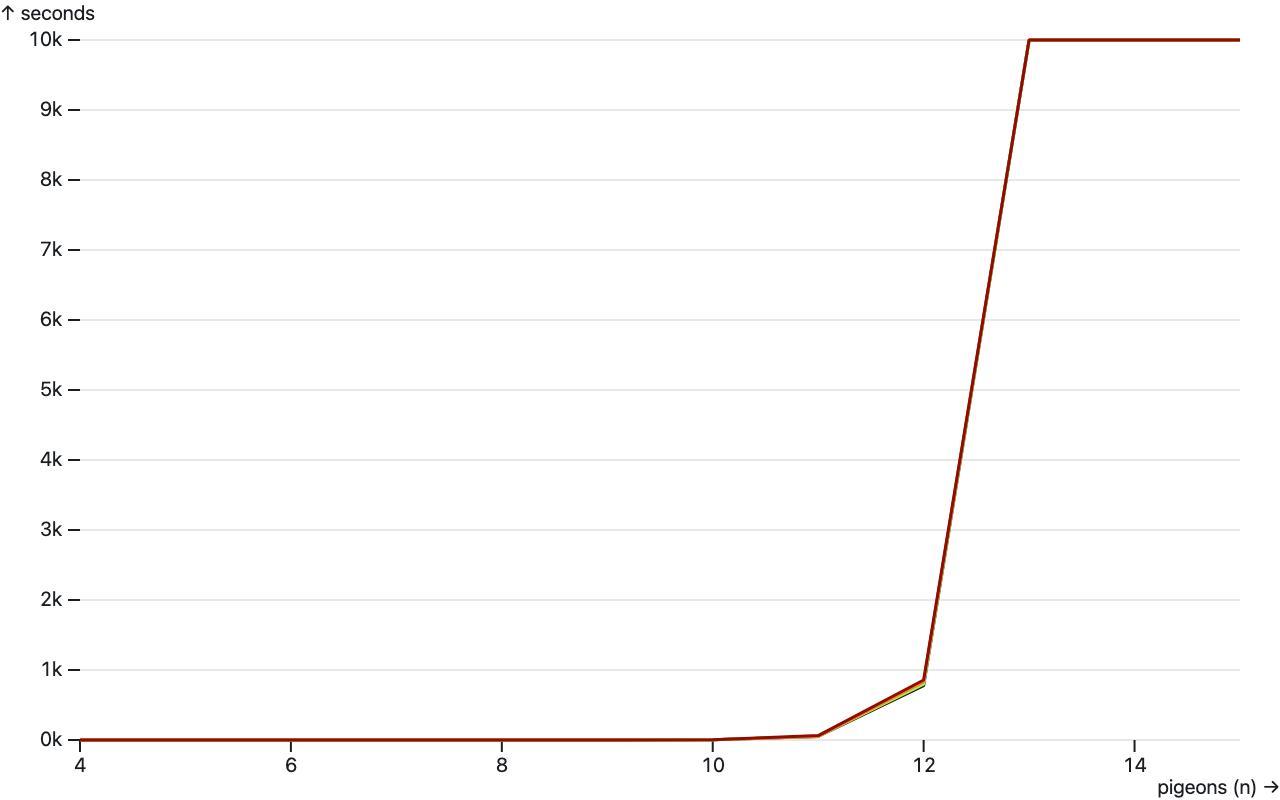
\includegraphics[width=0.75\textwidth]{pigeon-hole}
  \caption{\textbf{The relationship between the number of variables $n$ in the encoding of the Pigeon-hole SAT problem and the total solver time across 5 runs for all values $n = 4, 5, 6,...,15$. Solver runs were capped to 10,000 seconds.}}
  \label{fig:solver-times}
\end{figure}

\medskip
\noindent As we can see from the running times, we appear to hit an inflection point at $n = 12$ where solving times skyrocket and hit our maximum running time of 10,000 seconds. To assess the time complexity of running the SAT solver, we plot $n$ against $log(seconds)$. The results appear in Figure \ref{fig:solver-times-log}.

\begin{figure}
  \centering
  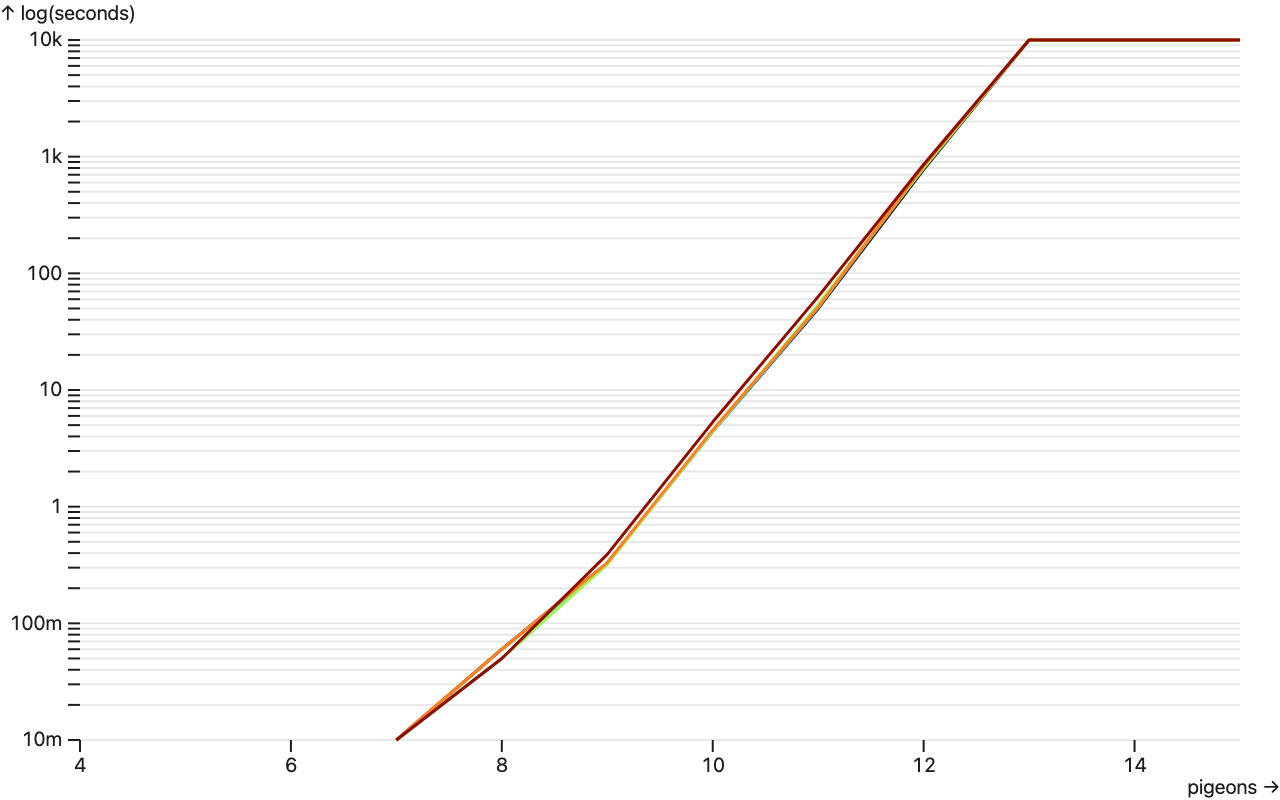
\includegraphics[width=0.75\textwidth]{pigeon-hole-log}
  \caption{\textbf{The relationship between the number of variables $n$ in the encoding of the Pigeon-hole SAT problem and $log(seconds)$ across 5 runs for all values $n = 4, 5, 6,...,15$. Solver runs were capped to 10,000 seconds.}}
  \label{fig:solver-times-log}
\end{figure}

\medskip
\noindent We can see that the relationship between $n$ and $log(seconds)$ is linear, suggesting that solving the Pigeon-hole problem takes the solver exponential time. If solving took polynomial time we would expect the relationship between $n$ and $log(seconds)$ to appear logarithmic rather than linear. This suggests that solving the Pigeon-hole problem is an especially difficult problem for SAT solvers.

\subsection{(b) BDDs}

\noindent The source code for my encoding of the Pigeon-hole SAT problem as a BDD is located in \code{hw1/bdds/hw1.py}.

\medskip
\noindent We see a similar relationship between $n$ and the running time of our BDD encoding of the Pigeon-hole SAT problem as we did with our DIMACS encoding; that is, determining satisfiability requires exponential time. Figure \ref{fig:bdd-pigeon-hole} shows the relationship between $n$ and the number of seconds to compute the BDD. One interesting difference between the two encodings is the significant difference in solving time. For example, for $n=12$ the BDD encoding took just 88 seconds to return UNSAT ($false$), while the CaDiCaL SAT solver took 775 seconds. When we plot $n$ againt $log(seconds)$, we notice the same linear relationship as was found when plotting $n$ against $log(seconds)$ for the DIMACS encoding. This shows that constructing the BDD still requires exponential time for the Pigeon-hole SAT problem. Figure \ref{fig:bdd-pigeon-hole-log} shows this relationship.

\begin{figure}
  \centering
  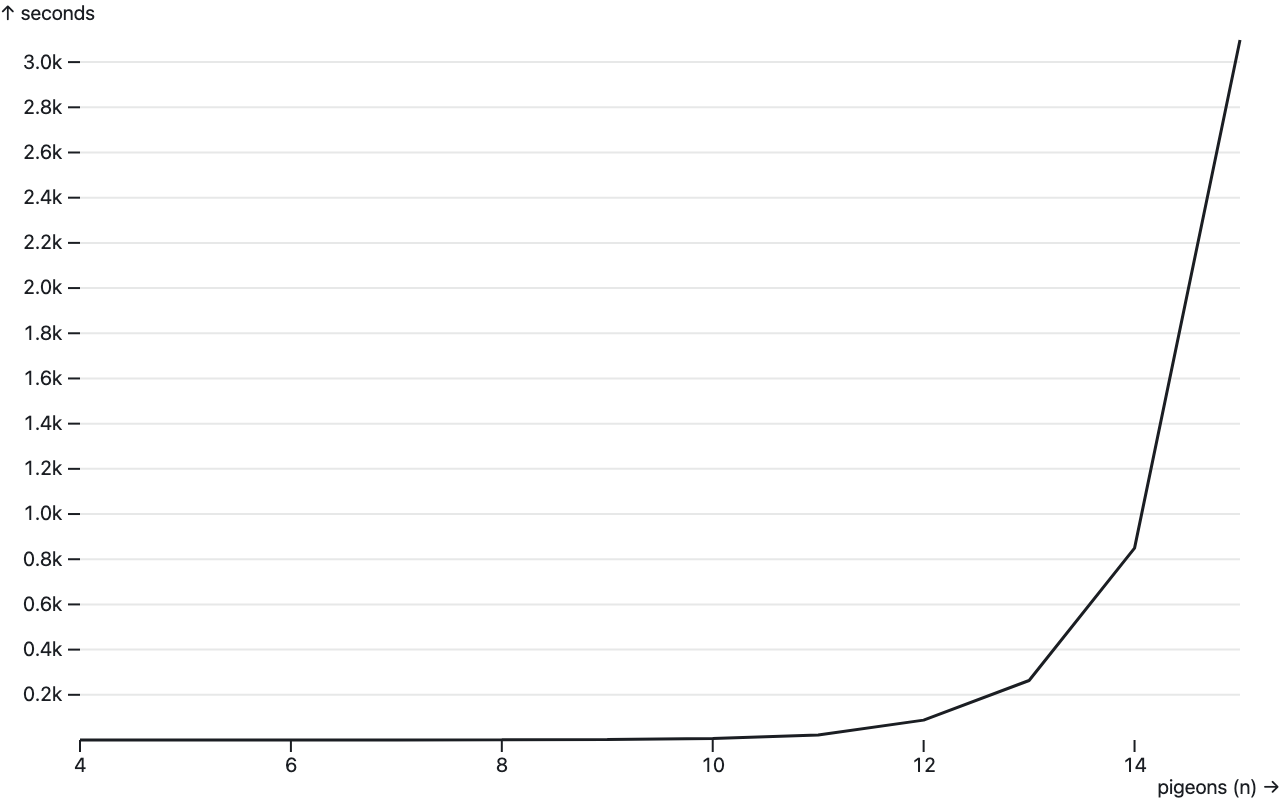
\includegraphics[width=0.75\textwidth]{bdd}
  \caption{\textbf{The relationship between the number of variables $n$ in the BDD encoding of the Pigeon-hole SAT problem and the number of seconds required to compute the BDD for all values $n = 4, 5, 6,...,15$.}}
  \label{fig:bdd-pigeon-hole}
\end{figure}

\begin{figure}
  \centering
  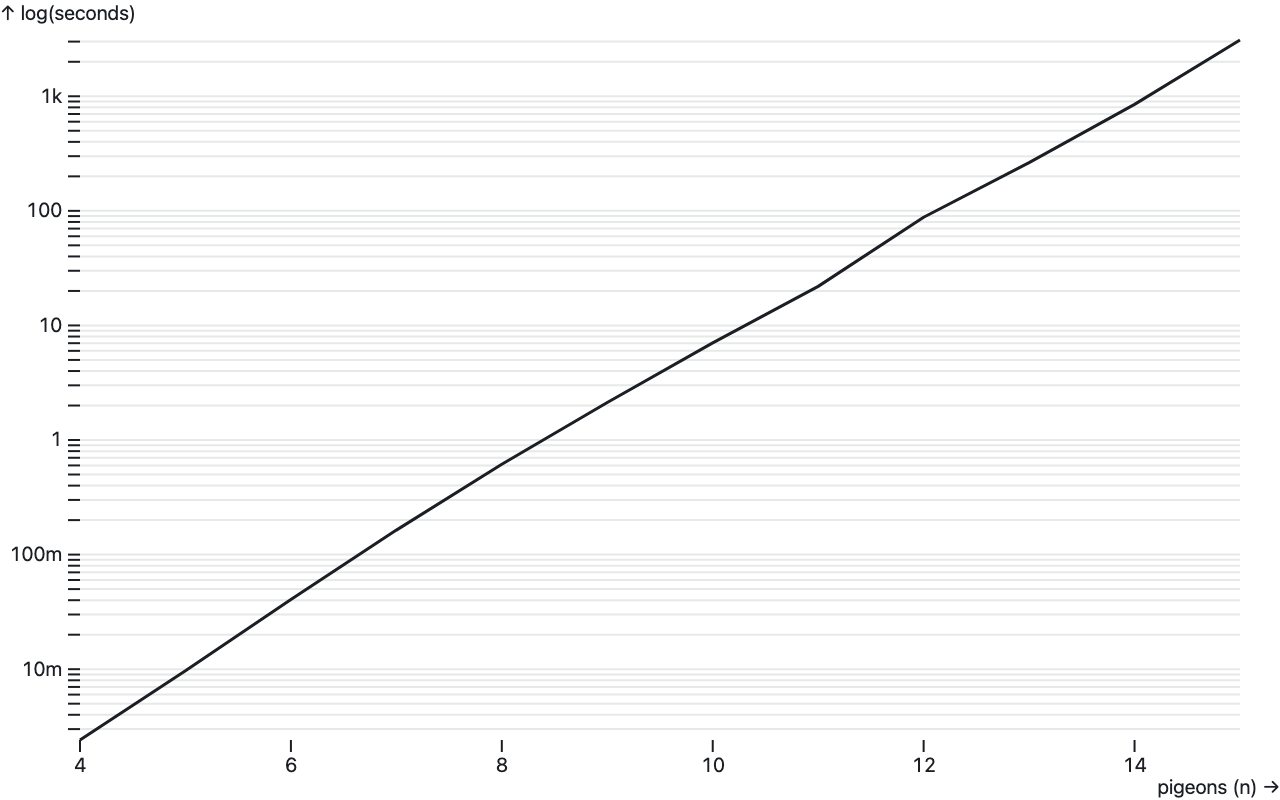
\includegraphics[width=0.75\textwidth]{bdd-log}
  \caption{\textbf{The relationship between the number of variables $n$ in the BDD encoding of the Pigeon-hole SAT problem and $log(seconds)$ required to compute the BDD for all values $n = 4, 5, 6,...,15$.}}
  \label{fig:bdd-pigeon-hole-log}
\end{figure}

\medskip
\noindent Applying dynamic reordering from the \code{dd} package by calling \code{bdd.configure(reordering=True)} did not appear to result in a difference in the runtime of the algorithm. While execution times increased somewhat comparted to invoking the algorithm without dynamic reordering, the pattern of exponential runtime remained the same. Figures \ref{fig:bdd-reorder} and \ref{fig:bdd-reorder-log} plot the results.


\begin{figure}
  \centering
  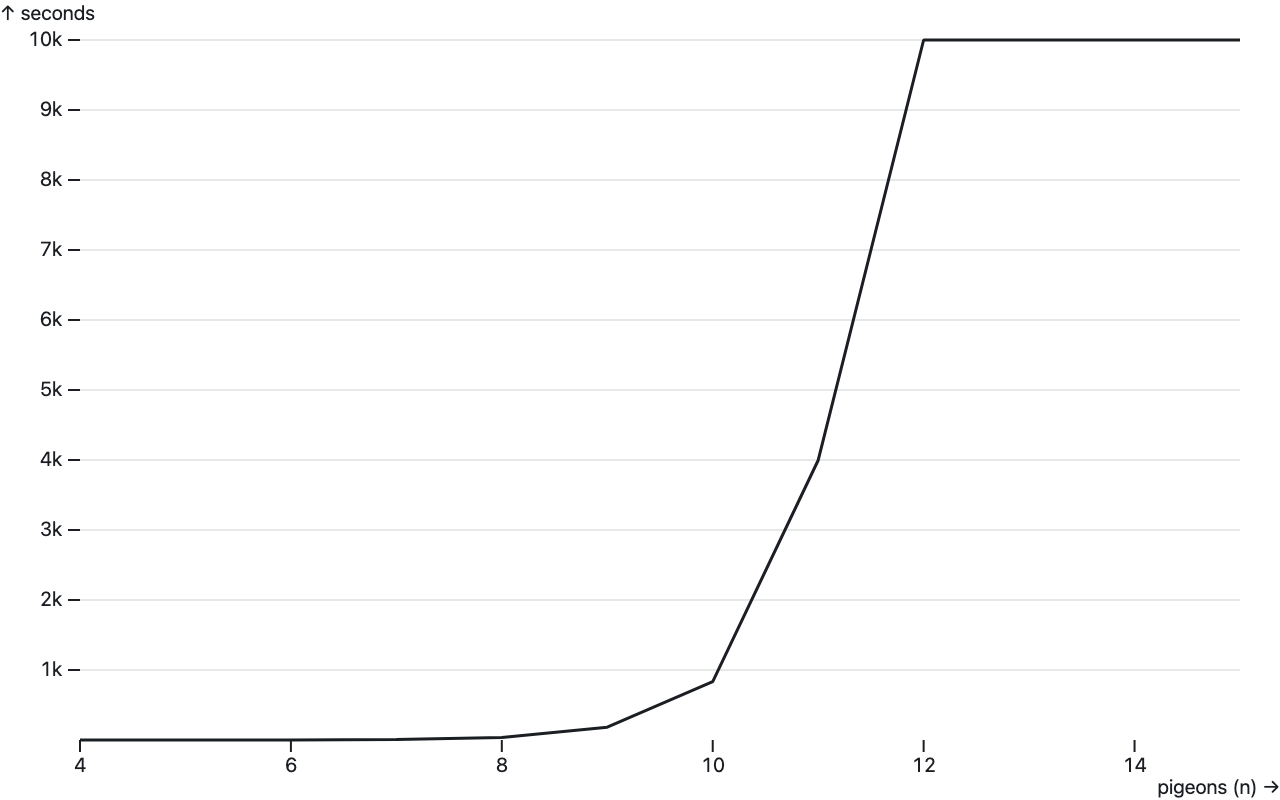
\includegraphics[width=0.75\textwidth]{bdd-reorder}
  \caption{\textbf{The relationship between the number of variables $n$ in the BDD encoding of the Pigeon-hole SAT problem and the number of seconds required to compute the BDD for all values $n = 4, 5, 6,...,15$ with dynamic reordering enabled. Similar to previous results we enforced a 10,000 second timeout.}}
  \label{fig:bdd-reorder}
\end{figure}

\begin{figure}
  \centering
  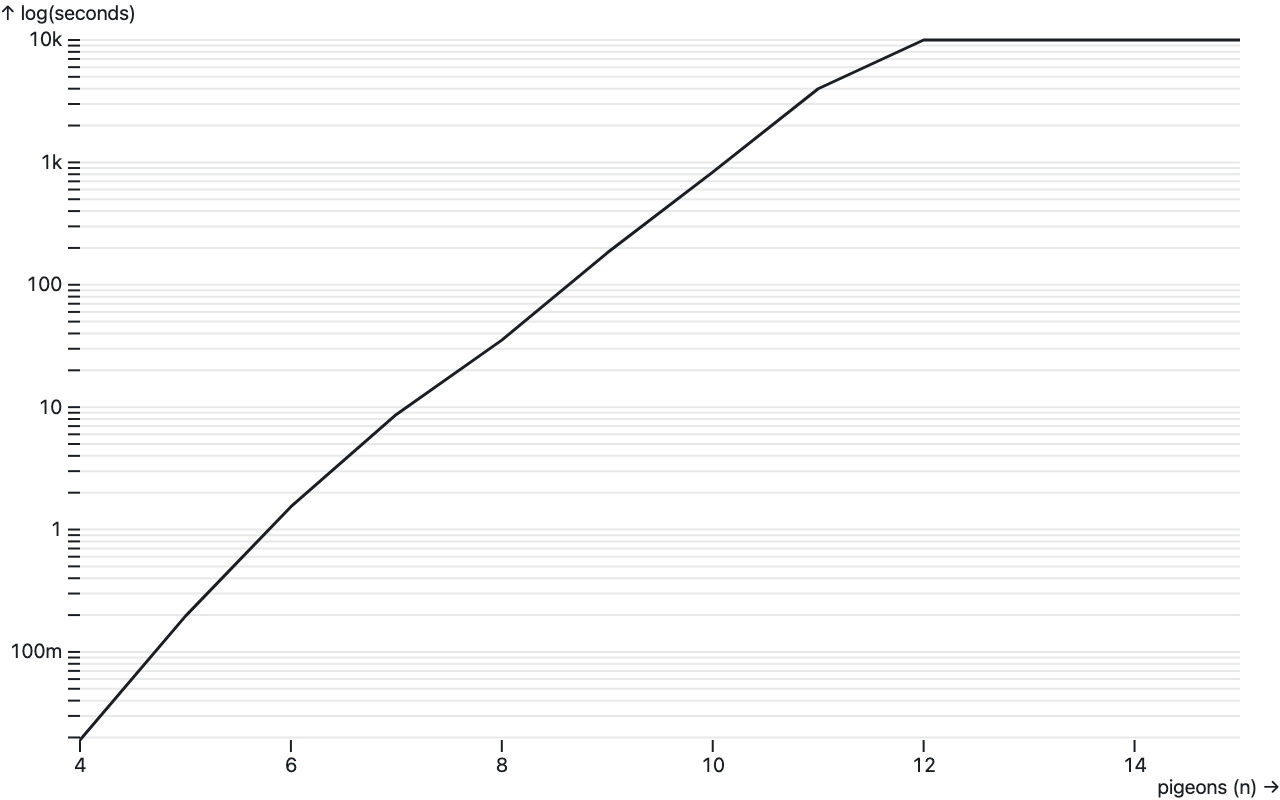
\includegraphics[width=0.75\textwidth]{bdd-reorder-log}
  \caption{\textbf{The relationship between the number of variables $n$ in the BDD encoding of the Pigeon-hole SAT problem and $log(seconds)$ required to compute the BDD for all values $n = 4, 5, 6,...,15$ with dynamic reordering enabled. Similar to previous results we enforced a 10,000 second timeout.}}
  \label{fig:bdd-reorder-log}
\end{figure}

\clearpage

\bibliographystyle{plain}
\bibliography{refs}

\end{document}
